\documentclass[12pt]{report}
\usepackage[utf8]{inputenc}
\usepackage{graphicx}
\usepackage{subcaption}
\usepackage{setspace}
\usepackage[english]{babel}
\usepackage{wrapfig}
\usepackage[font=small,labelfont=bf]{caption}
\usepackage{amsmath}

\doublespacing

\graphicspath{{Images/}}
\title{Thesis}
\author{John DeCorato}
\date{ }

\setlength{\parindent}{3em}
\setlength{\parskip}{1em}

\begin{document}

\chapter{Creating a Sketch}

The most basic operation in any sketch-based modeling system is, of course, obtaining a sketch from the user.
The key characteristic of a sketch-capable input device is that it allows freehand input.
While a mouse is capable of this form of input, devices that more closely mimic the feel of freehand drawing using a pen, such as a digitizing tablet, are better for users to maximize their ability to draw.
Devices that are both an input device and a display are particularly suited to this, because it most closely mimics traditional artist creation methods by allowing direct interaction with the sketch space, as opposed to Wacom tablets where the space is relative

\begin{figure}
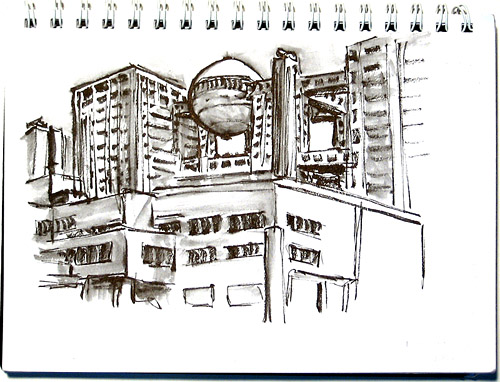
\includegraphics[width=0.7\textwidth]{fujitv}
\caption{An example of a sketch}
\end{figure}

Pencil and paper is a rich communication method. 
Artists convey information not only with the shape of the completed objects in the sketch, but also through more subtle methods such as pressure and stroke style.
Small details can relay information about the object, such as important details; heavier lines or many small strokes usually show more focus was put in a particular area.

\section{Representation of a Sketch}

At the bare minimum, an input device will provide positional information in some two dimensional coordinate system, usually one based on the interaction window.
This information represents a piecewise linear approximation of continuous movement.
Sampling rates vary from one device to the next.
The samples themselves may also be spaced irregularly, with sample points closer as users draw slowly or carefully.

\begin{figure}
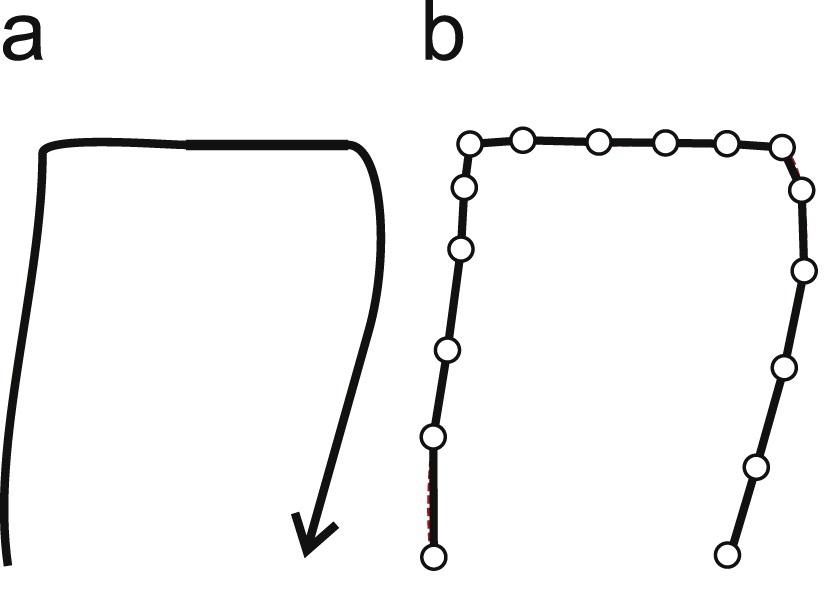
\includegraphics[width=0.7\textwidth]{stroke}
\caption{An input stroke (a) is provided to the application as (b) a sequence of point samples. The point samples represent a piecewise linear approximation of the original sketch.}
\end{figure}

We will refer to this sampled sequence of points as a stroke. 
Strokes are stored as a list of points, objects containing coordinates from the sample space, sorted by time.
A sketch is comprised of a large number of these stroke objects.

Strokes can be organized in order to enhance the drawing experience as well as minimize clutter when working on complicated images.
The most common sorting method is a layer, an object that contains a subset of strokes from the total image.
Layers are naturally contained in a hierarchical data structure. 
If two layers have a stroke with a point at the same space, then the layer higher in the hierarchy is displayed.
It is similar to stacking sheets of transparent tracing paper.
Layers can be turned on or off to toggle whether or not they are displayed.
This functionality is useful for focusing on specific ares on the sketch.

To summarize, a sketch contains any number of layers.
These layers are put in a list, and ordered by the user.
Each layer contains a number of strokes created by drawing with a pen input device, and each stroke contains a series of points sampled from the sketch input.

\section{Spline Curves}

As stated in the previous section, a stroke object contains a linear approximation of the input from the user. 
While this would work decently well assuming we are working with a static raster image, three dimensional sketching allows the user to move the camera.
If the camera were zoomed in close enough, the linear approximation of the stroke would no longer look like the original input, instead appearing like long connected line segments.
To remedy this, a mathematical representation of the curve is needed.
In computer graphics, this is commonly accomplished with spline curves.

A spline is a collection of polynomial segments.
These segments can be linear, cubic, or any degree polynomial function.
Splines are a common solution for modeling smooth curves from a small number of points.

For this project, we use a Bézier curve function for the spline pieces.
A Bézier curve is a parametric curve commonly used in computer graphics to model infinitely scaling, smooth curves.
The curve is defined by control points P0, P1, ..., Pn, and is explicitly evaluated as follows:
\begin{align}
  \mathbf{B}(t) = {} &\sum_{i=0}^n {n\choose i}(1 - t)^{n - i}t^i\mathbf{P}_i \\
                = {} &(1 - t)^n\mathbf{P}_0 + {n\choose 1}(1 - t)^{n - 1}t\mathbf{P}_1 + \cdots \\
                  {} &\cdots + {n\choose n - 1}(1 - t)t^{n - 1}\mathbf{P}_{n - 1} + t^n\mathbf{P}_n,\quad 0 \le t \le 1
\end{align}
where $\scriptstyle {n \choose i}$ are the binomial coefficients, defined as
\begin{equation}
\binom nk = \binom{n-1}{k-1} + \binom{n-1}k \quad \text{for all integers }n,k : 1\le k\le n-1
\end{equation}
with initial values 
\begin{equation}
\binom n0 = \binom nn = 1 \quad \text{for all integers } n\ge0
\end{equation}
The curve can also be evaluated recursively, by
\begin{align}
\mathbf{B}_{\mathbf{P}_0}(t) = \mathbf{P}_0 \\
\mathbf{B}(t) = \mathbf{B}_{\mathbf{P}_0\mathbf{P}_1\ldots\mathbf{P}_n}(t) = (1-t)\mathbf{B}_{\mathbf{P}_0\mathbf{P}_1\ldots\mathbf{P}_{n-1}}(t) + t\mathbf{B}_{\mathbf{P}_1\mathbf{P}_2\ldots\mathbf{P}_n}(t)
\end{align}
What this equation means is that a Bezier spline of order $n$ can be defined by linear interpolation between two splines of order $n - 1$.

The most commonly used curves are linear, quadratic, and cubic interpolations, where n = 1 for linear, 2 for quadratic, and 3 for cubic.
Evaluating n = 1 gives us: 
\begin{align}
\mathbf{B}(t)=\mathbf{P}_0 + t(\mathbf{P}_1-\mathbf{P}_0)=(1-t)\mathbf{P}_0 + t\mathbf{P}_1 \mbox{ , } 0 \le t \le 1
\end{align}
which is linear interpolation.


For this project, we will use a cubic Bézier function for the spline segments.
Four points P0, P1, P2 and P3 in the space define a cubic Bézier curve. 
The curve starts at P0 going toward P1 and arrives at P3 coming from the direction of P2. 
Usually, it will not pass through P1 or P2; these points are only there to provide directional information. 
The distance between P0 and P1 determines the magnitude and velocity the curve moves towards P1 before turning towards P2.


The cubic spline curve is explicitly defined as:
The explicit form of the curve is:
\begin{align}
\mathbf{B}(t)=(1-t)^3\mathbf{P}_0+3(1-t)^2t\mathbf{P}_1+3(1-t)t^2\mathbf{P}_2+t^3\mathbf{P}_3 \mbox{ , } 0 \le t \le 1.
\end{align}
For some choices of P1 and P2 the curve may intersect itself, or contain a cusp.
The derivative of the cubic Bézier curve with respect to t is
\begin{align}
\mathbf{B}'(t) = 3(1-t)^2(\mathbf{P}_1 - \mathbf{P}_0) + 6(1-t)t(\mathbf{P}_2 - \mathbf{P}_1) + 3t^2(\mathbf{P}_3 - \mathbf{P}_2) \,.
\end{align}
The second derivative of the Bézier curve with respect to t is
\begin{align}
\mathbf{B}''(t) = 6(1-t)(\mathbf{P}_2 - 2 \mathbf{P}_1 + \mathbf{P}_0) +  6t(\mathbf{P}_3 - 2 \mathbf{P}_2 + \mathbf{P}_1) \,.
\end{align}

If we want our spline to closely approximate the sketch, we have two options. 
First, we can generate a spline curve that passes through our control points in order, by splitting the input set into subsets of 4 control points.
Any series of any 4 distinct points can be converted to a cubic Bézier curve that goes through all 4 points in order.
Given the starting and ending point of some cubic Bézier curve, and the points along the curve corresponding to t = 1/3 and t = 2/3, the control points for the original Bézier curve can be recovered.
Adjacent sections would contain a duplicate point for the Bézier curve generation.

\paragraph{Pros}

\begin{itemize}
\item This method is guaranteed to go through every point sampled from the input curve
\item The memory use from generating the curve is linearly related to the number of control points.
\end{itemize}

\paragraph{Cons}
\begin{itemize}
\item If the sample distance changes dramatically, the generated curve contains artifacts that make it appear to not look like a curve that would be drawn intentionally.
\item If the number of point is not $mn + 1$, where $m$ is one less than the number of points per curve generated, sub-cases must be made. If there is one point left over, then the last piece generated will be a line segment.
\end{itemize}

\begin{center}
\begin{figure}
\begin{center}
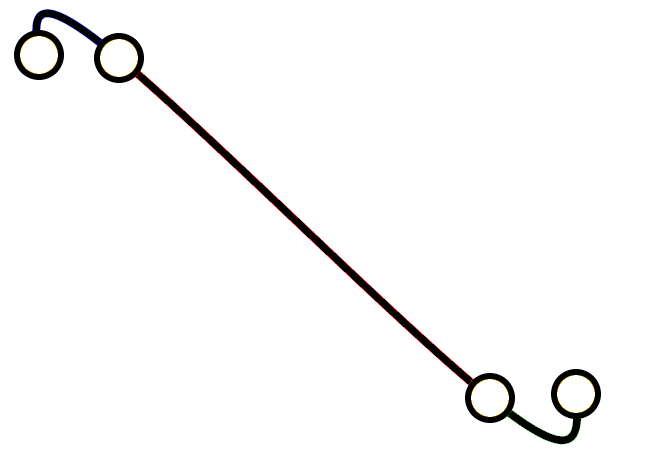
\includegraphics[width=0.8\textwidth]{splineartifact}
\end{center}
\caption{An example of an artifact in the spline generation caused by oddly spaced sample points. This effect would be exasperated while zooming in on the curve.}
\end{figure}
\begin{figure}
\begin{center}
\includegraphics[width=0.9\textwidth]{terminationbspline}
\end{center}
\caption{Using the distance from the control points for termination.}
\end{figure}
\end{center}

The second approach is we can use the input samples as control points to generate a piecewise spline curve. 

\paragraph{Pros}

\begin{itemize}
\item This method works with any curve which contains more than 5 sample points.
For input with less than 5 points, a Bézier curve can be generated, using a linear, quadratic, and cubic curve for input with 2, 3, or 4 sample points respectively.
\item This method is better at dealing with extreme changes in sample rates because the produced curve contains less convex and concave changes. However, it is likely that the produced curve will still be inaccurate.
\end{itemize}

\paragraph{Cons}
\begin{itemize}
\item The curve generated will not pass through the sampled points. However, if the sample rate is high, it will be close.
\end{itemize}

In practice, not generating a curve that is exactly the same as the input sample points is not as necessary as one would think. 
The most important part is the curve should match the form of the original curve.
If the detail of the curve is important, then the user will probably draw more slowly, allowing for a greater number of sample points, and generating a spline that closely resembles the shape of the detailed section.
The simpler and more consistent shape of the recursive B-spline curve makes it a better choice than the inverse control point calculation, as seem in practice by a large number of applications implementing spline approximations, including Mischief.

\subsection{Algorithm}

We begin with a list of control points, numbered from 0 to N-1. 
Segment i of the curve is influenced by control points i-1, i, i+1, and i+2.
Using this definition we can generate N-3 segments from the N control points without falling off the ends of the sequence.

Since we can't render a spline, we need to approximate the curve by subdividing it into small line segments.
We're going to divide each Bezier curve into a set of connected linear components, with the intent that a large enough number will look sufficiently smooth.
Subdivision of these segments occurs as follows:
\begin{enumerate}
\item Begin with points $\{P_0,P_1,P_2,P_3\}$, which define a Bézier curve, and a number $u, 0 \le u \le 1$
\item Define $L_1=(P_0 + P_1)*u$, $H=(P_1 + P_2)*u$, and $R_2=(P_2 + P_3)*u$
\item Define $L_2=(L_1 + H)*u$, and $R_1=(H + R_2)*u$
\item Define $M=(L_2 + R_1)*u$
\item Create two new Bézier curves using $\{P_0,L_1,L_2,M\}$ and $\{M,R_1,R_2,P_3\}$
\item Repeat steps 2 through 5 until a termination criteria is met. Possible criteria include distance between control points, and distance between control points $P_1$ and $P_2$ and the line between $P_0$ and $P_3$.
\end{enumerate}
If the termination criteria is small enough, then the curve will appear very smooth, even when zooming in to the curve.

The complete algorithm is as follows:

$TODO: bug joe about writing in algorithm format$

This algorithm produces a smooth B-spline curve starting at control point 0 and ending at N-1.






\end{document}